\documentclass{standalone}
\usepackage{tikz}
\usepackage{ctex,siunitx}
\usepackage{tkz-euclide}
\usepackage{amsmath}
\usetikzlibrary{patterns, calc}
\usetikzlibrary {decorations.pathmorphing, decorations.pathreplacing, decorations.shapes,}
\begin{document}
\small
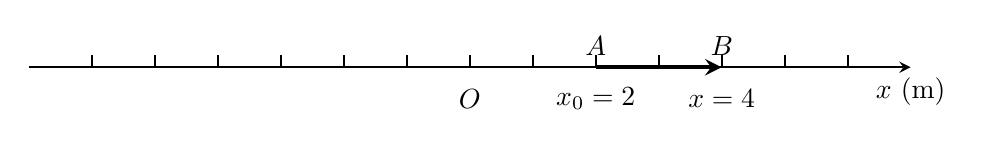
\begin{tikzpicture}[>=stealth, thick,scale=0.8]
  \draw [->](0,0) --(14,0)node [below]{$x$ (\unit{m})} ;
  \foreach \x in {1,2,...,13}
  {
    \draw (\x, 0)--(\x,.2);
  }
  \node at (7,-.5){$O$}; \node at (9,-.5){$x_0=2$}; \node at (11,-.5){$x=4$}; 
  \draw[->, ultra thick] (9,0) node [above]{$A$}--(11,0)node [above]{$B$};
\end{tikzpicture}
\end{document}